\begin{figure}[H]
	\centering
\begin{subfigure}{0.32\textwidth}
	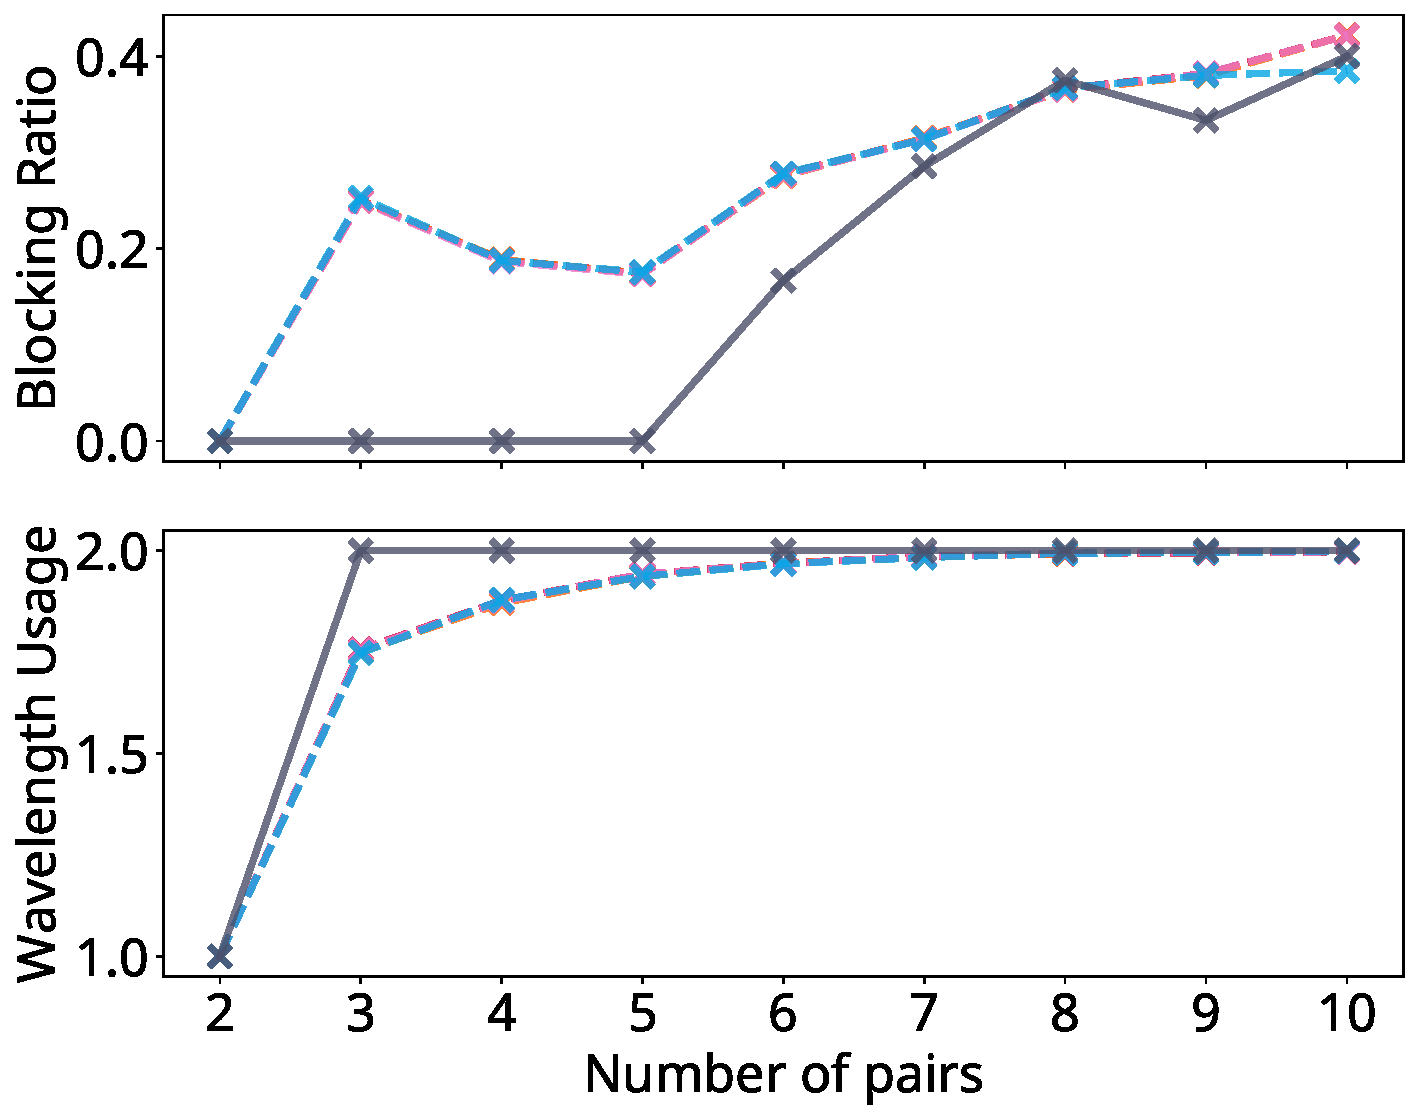
\includegraphics[width=\textwidth]{pictures/plots/n_pairs/cc/x-1-2-s.pdf}
	\caption{\scriptsize $N=1, \abs{\Lambda} = 2$, small topology}
\end{subfigure}
\begin{subfigure}{0.32\textwidth}
	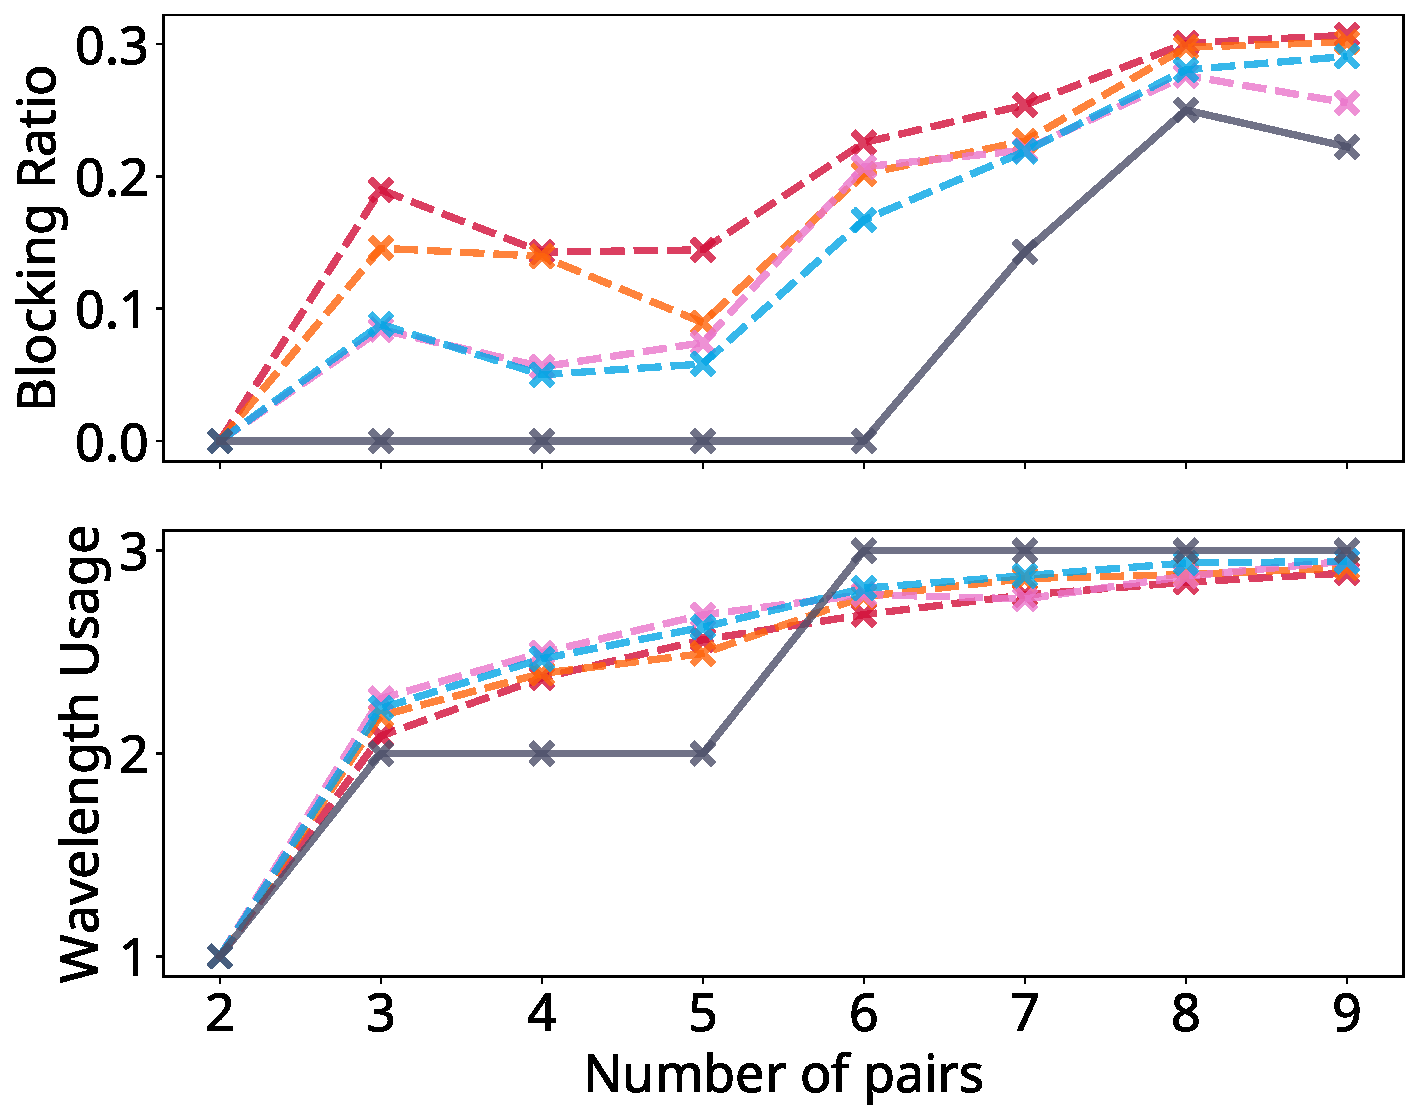
\includegraphics[width=\textwidth]{pictures/plots/n_pairs/cc/x-1-3-s.pdf}
	\caption{\scriptsize $N=1, \abs{\Lambda} = 3$, small topology}
\end{subfigure}
\begin{subfigure}{0.32\textwidth}
	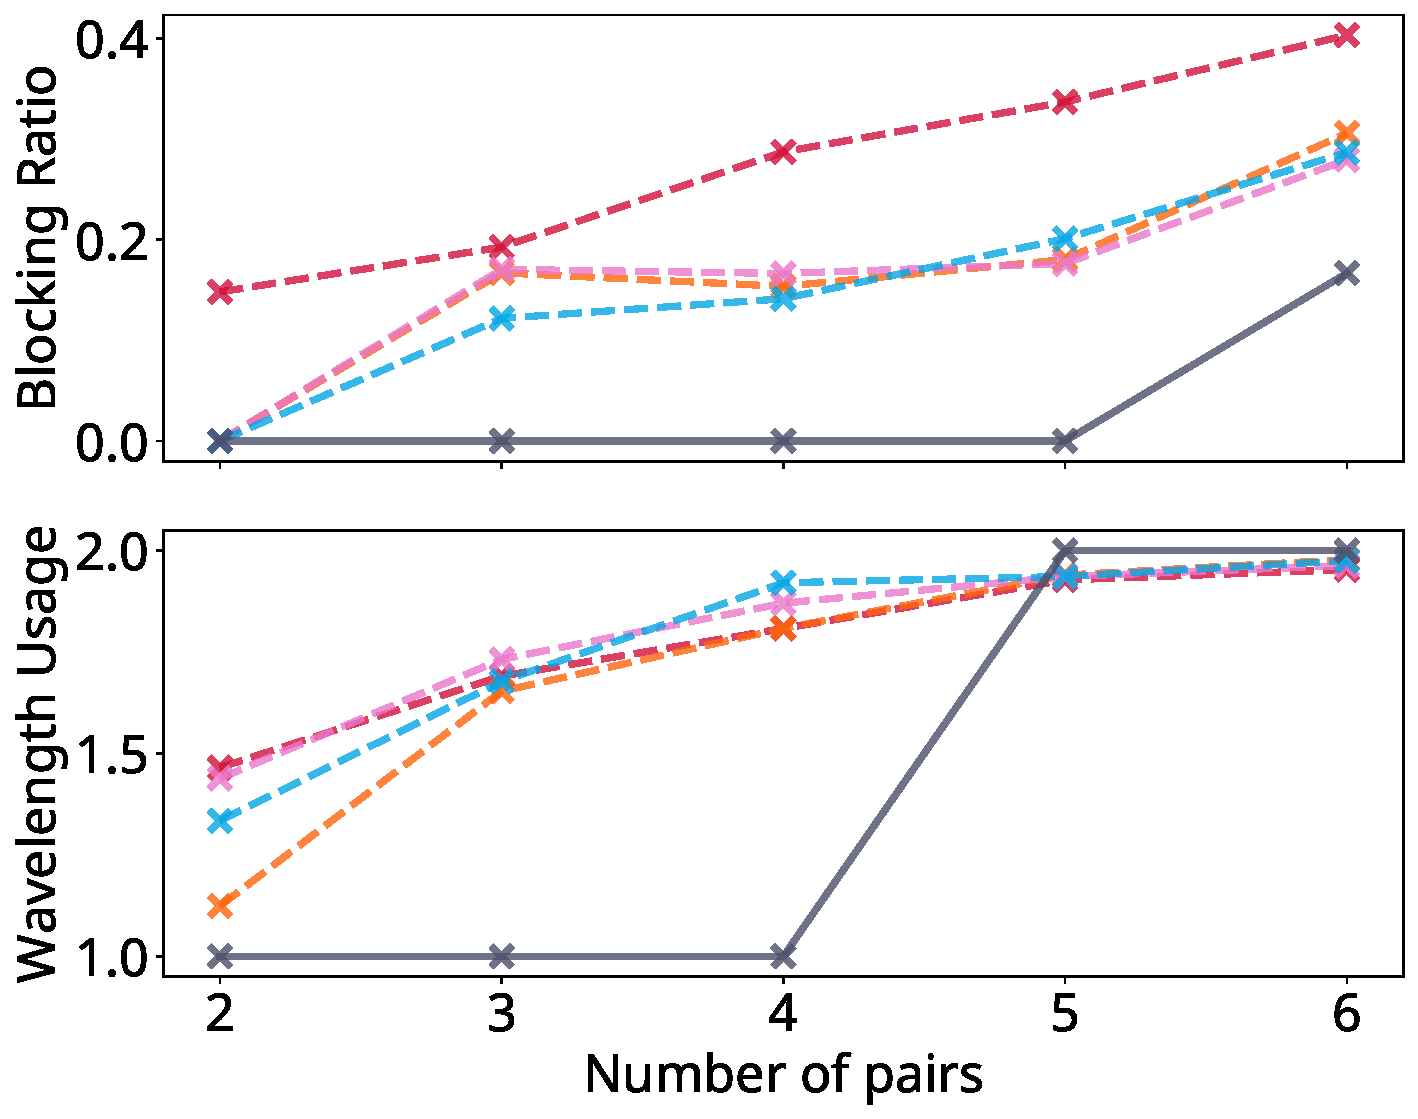
\includegraphics[width=\textwidth]{pictures/plots/n_pairs/cc/x-2-2-s.pdf}
	\caption{\scriptsize$N=2, \abs{\Lambda} = 2$, small topology}
\end{subfigure}
% \caption{The blocking probability and number of wavelength used.
% \protect\reddashed represents $p=1$
% \protect\peachdashed represents $p=2$
% \protect\pinkdashed represents $p=3$
% \protect\skydashed represents $p=4$
% \protect\blackline represents SPFF
% }
% \caption{\scriptsize After}
\label{fig:cc_pairs}
\end{figure}
